\documentclass{report}

\usepackage[UTF8]{inputenc}
\usepackage[T1]{fontenc}
\usepackage[francais]{babel}
\usepackage{graphicx}
\usepackage{fullpage}
\usepackage{eurosym}

\title{\textbf{{\huge Fiche de la Gestion qui tue sa mère}}}
\author{Jean-Pierre \bsc{Mohamed}}
\date{12 novembre 2014}

\begin{document}
 
\maketitle

\chapter{Introduction}

\emph{"Le temps est une ressource rare, donc si vous n'êtes pas attentifs, je peux revenir à mon état de stabilité : ne rien faire."} - Jean MARQUET
\\ \\

\emph{"Bienvenue et bon courage pour le test..."} - Jean-Luc KRUST

\chapter{Les Budgets}

\paragraph*{Prévision :} Les prévisions sont les objectifs et la planification d'une entreprise.

\paragraph*{Budget :} Un budget est  un compte prévisionnel de l'entreprise. Il est constitué d'un compte de résultat prévisionnel et d'un bilan prévisionnel.

\paragraph*{Programme :}
Un programme est une évaluation prévisionnelle des objectifs en quantité d'une entreprise.

\paragraph*{Budget : }
Un budget est une évaluation prévisionnelle en valeur des objectifs d'une entreprise.

\paragraph*{Établir le programme des Ventes :}
{\Large$ \frac{Chiffre\ d'affaire}{Prix\ unitaire} $}

\paragraph*{Établir le budget des Ventes :}
$ Quantite \ vente \times Prix\ unitaire \times TVA$

\paragraph*{Établir le programme des Approvisionnements :}
Prendre la formule suivante : 
\\ $Stock\ initial + Achat = Vente + Stock Final$ puis trouver la partie "Achat"

\paragraph*{Établir le budget des Approvisionnement :}
A partie de la partie "Achat", faire : 
\\$Achat \times Prix\ unitaire \times  TVA$

\paragraph*{Déterminer la trésorerie net :}
$Tresorerie\ net = Total\ encaissement - Total\ décaissement$

\paragraph*{Déterminer le résultat :} 
$Resultat = Total\ produits - Total\ charges$
\\Si le total des produits est plus grand que le total des charges, alors l'entreprise est rentable, sinon elle est en déficit.

\paragraph*{Soumission à la TVA :}
Dans une entreprise les achats, les ventes, les charges externes et les services bancaires sont soumis à la TVA. Les salaires, les impôts et les Intérêts ne sont pas soumis à la TVA.

\paragraph*{Variation de la trésorerie et du résultat :}
Un achat au comptant de marchandises diminue la trésorerie et le résultat.
\\ Un investissement à crédit ne diminue aucun des deux.
\\ L'amortissement d'une machine diminue le résultat.


\chapter{La TVA}

\paragraph*{Définition de la TVA :}
La taxe sur la valeur ajoutée (T.V.A.) est un impôt général de consommation qui atteint la plupart des biens et services consommés en France. C’est donc le consommateur final qui supporte la T.V.A. L'entreprise a un rôle d'intermédiaire entre le consommateur final et l'État.

\paragraph*{TVA collectée :} La TVA collectée est inclus dans les ventes. Ce montant de TVA collectée doit être reversé à l'État. L'organisation a donc une dette envers l'État tant que la TVA collectée n'a pas été reversée à l'État.

\paragraph*{TVA déductible :} La TVA déductible est inclus dans les achats. L'organisation a une créance envers l'État tant que la TVA déductible n'a pas été récupérée.

\paragraph*{TVA à décaisser :} Si la TVA collectée est supérieure à la TVA déductible, l’organisation a une dette envers l’État. Cette dette se nomme TVA à décaisser.

\paragraph*{Crédit de TVA :} Si la TVA collectée est inférieure à la TVA déductible, l’organisation a une créance envers l’État. Cette créance se nomme crédit de TVA.
\\

\begin{center}
Résumé en image
\end{center}

\begin{figure}[h]
\begin{center}
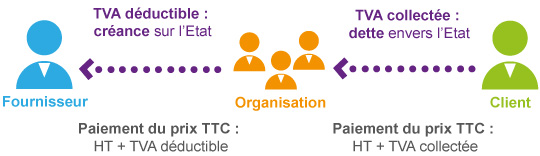
\includegraphics[scale=0.75]{TVA.jpg}
\end{center}
\end{figure}

\newpage

\paragraph*{Passer d'une valeur HT à une valeur TTC :}
Formule 1 : $Valeur\ TTC =  Valeur\ HT + TVA$
\\Formule 2 : $TVA = Valeur\ HT \times Taux\ de\ TVA$
\\Formule générale : $Valeur\ TTC = Valeur\ HT \times  (1 + Taux\ de\ TVA)$

\paragraph*{Passer d'une valeur TTC à une valeur HT :}
$Valeur\ HT = \frac{Valeur\ TTC}{ 1 + Taux\ de\ TVA}$

\paragraph*{Retrouver le montant de TVA à partir d'une valeur TTC :}
$TVA = (\frac{Valeur\ TTC}{1 + Taux\ de\ TVA}) \times Taux\ de\ TVA$

\chapter{Capitalisation et actualisation}

\paragraph*{Capitalisation :} La capitalisation permet de déterminer la valeur future d'une somme placée à un taux d'intérêt. Elle est l'opération inverse de l'actualisation.

\paragraph*{Actualisation :} L'actualisation consiste à déterminer la valeur d'aujourd'hui de flux qui se produiront dans le futur : elle est donc l'inverse de la capitalisation. Elle permet de comparer des sommes reçues ou versées à des dates différentes.

\paragraph*{Taux d'intérêt :} Le taux d'intérêt permet de mesurer la préférence pour le présent.
\\ La formule :{\Large $(\frac {Capital \times Taux\ annuel\ interet}{12}) \times Le\ nombre\ de\ mois\ des\ depots$}

\paragraph*{Valeur acquise :}
$Capital + interets$

\paragraph*{Effet de commerce :} L'effet de commerce est un papier qu'on signe pour que le client reconnaisse qu'il doit devoir la somme des marchandises achetées par crédit. Cette effet de commerce peut être utilisé pour acheter des biens chez un autre fournisseur.

\paragraph*{Agios :}
$(\frac{Duree}{360}) \times Taux\ annuel\ escompte \times Somme\ nominale + Commision\ HT$

\paragraph*{Bordereau d'escompte :}
$Somme\ nominale - (Agrios + TVA)$

\paragraph*{Taux Effectif Global (TEG) :} Le TEG est un coût de financement.
\\
{\Large$(\frac{Agios \times \frac{360}{Duree}}{Somme\ nominale}) \times 100$}

\chapter{Placement et emprunts à court terme et long terme}

\section{Pour la capitalisation (Savoir la somme dans le futur)}

\paragraph{Valeur acquise par un capital C placé au taux t pendant n périodes.} 
Cette méthode consiste à mettre qu'une somme et laisser faire les taux d'intérêts pour voir la somme qu'on aura à une date donnée.
\\ La formule : $C \times (1 + t)^{n}$

\paragraph{Valeur acquise par une suite de n annuités constantes x placées au taux t immédiatement après le versement de la dernière annuité.}
Cette méthode consiste à savoir la somme qu'on aura à une date définie en mettant une somme fixe tous les mois additionnée avec les taux d'intérêts .
\\La formule : {\Large$X \times \frac{(1 + t)^{n} -1}{t}$}

\section{Pour l'actualisation (Connaitre la somme à mettre pour avoir le somme finale qu'on souhaite)}

\paragraph{Valeur actuelle d'un capital C disponible dans n périodes aux taux d'actualisation t.} 
Cette méthode permet de connaitre la somme à mettre au départ lorsqu'on veut avoir une somme finale précise avec les taux d'intérêts.
\\La formule : $C \times (1 + t)^{-n}$

\paragraph{Valeur actuelle au taux d'actualisation t d'une suite de n annuités constantes x une période avant le 1er versement}
Cette méthode consiste à connaitre la somme à mettre lorsqu'on veut avoir une somme final précise avec les sommes versées chaque mois et les taux d'intérêts.
\\La formule : {\Large $X \times \frac{1 - (1 + t)^{-n} }{t}$}

\chapter{Les choix d'investissement}

\paragraph{Flux Net de Trésorerie d'Exploitation (FNTE) :}
 $Resultat\ net + Amortissements + Reserve (Provisions)$
 
 \paragraph{Valeur actuelle nette (VAN) :}
La valeur actuelle nette est un flux de trésorerie actualisé représentant l'enrichissement supplémentaire d'un investissement par rapport au minimum exigé par les apporteurs de capitaux.
\\La formule : $- (Cout\ du\ projet) + FNTE \times$ {\Large $\frac{1 - (1 + t)^{-n}}{t}$} 

\paragraph{Taux de Rendement Interne (TRI) :}
Le taux de rentabilité interne ou TRI d'un investissement est synonyme du taux de rentabilité de cet investissement. En clair c'est le taux d'actualisation pour lequel la valeur actuelle nette de l'investissement est nulle. 
\\La formule : $R1 + (( R2- R1) \times${\Large $ \frac{VAN1}{VAN1 + VAN2})$}
\\R1 et R2 représente le résultat de VAN1 et VAN2 avec la formule du VAN. VAN1 et VAN2 représente les taux (Exemple : VAN15\% et VAN16\%).
\\ATTENTION : ne pas oublier de convertir les pourcentages en décimales. 

\paragraph{Délai de Récupération du Capital Investi (DRCI) :}
Le délai de récupération, ou pay-back ratio, mesure le temps nécessaire à la récupération du montant initial d'un investissement en le comparant aux flux cumulés de trésorerie.
Exemple : mon coût de projet est de 1000\euro\ et mon FNTE annuel est de 300\euro\ . Il me faut donc 3ans et 1/3 d'une année pour avoir mon DCRI.

\paragraph{Indice de Profitabilité (IP) :}
L'indice de profitabilité ou de rentabilité est égal au ratio de la valeur actuelle nette des flux de trésorerie d'exploitation sur la valeur actuelle nette des flux d'investissement. 
\\La formule :{\Large  $\frac{VAN}{Cout\ du\ projet}$}$\times 100$

\end{document}

